\section{Parallelization}
% Keywords: MPI, spatial domain geometry, communication surface, 6 facets, world geometry, 
Since there are no long range forces, each collision cell is completely independent of the other cells. We can then divide the spatial domain into subdomains, each fully controlled by one processor. Each processor is responsible for executing the timestep for each particle that are in the corresponding volume. The processors will usually contain many collision cells as illustrated in figure \ref{fig:dsmc_parallelization_1}. We will use the terms \textit{processor}, \textit{node} and \textit{CPU} interchangeably.
\begin{figure}[h]
\begin{center}
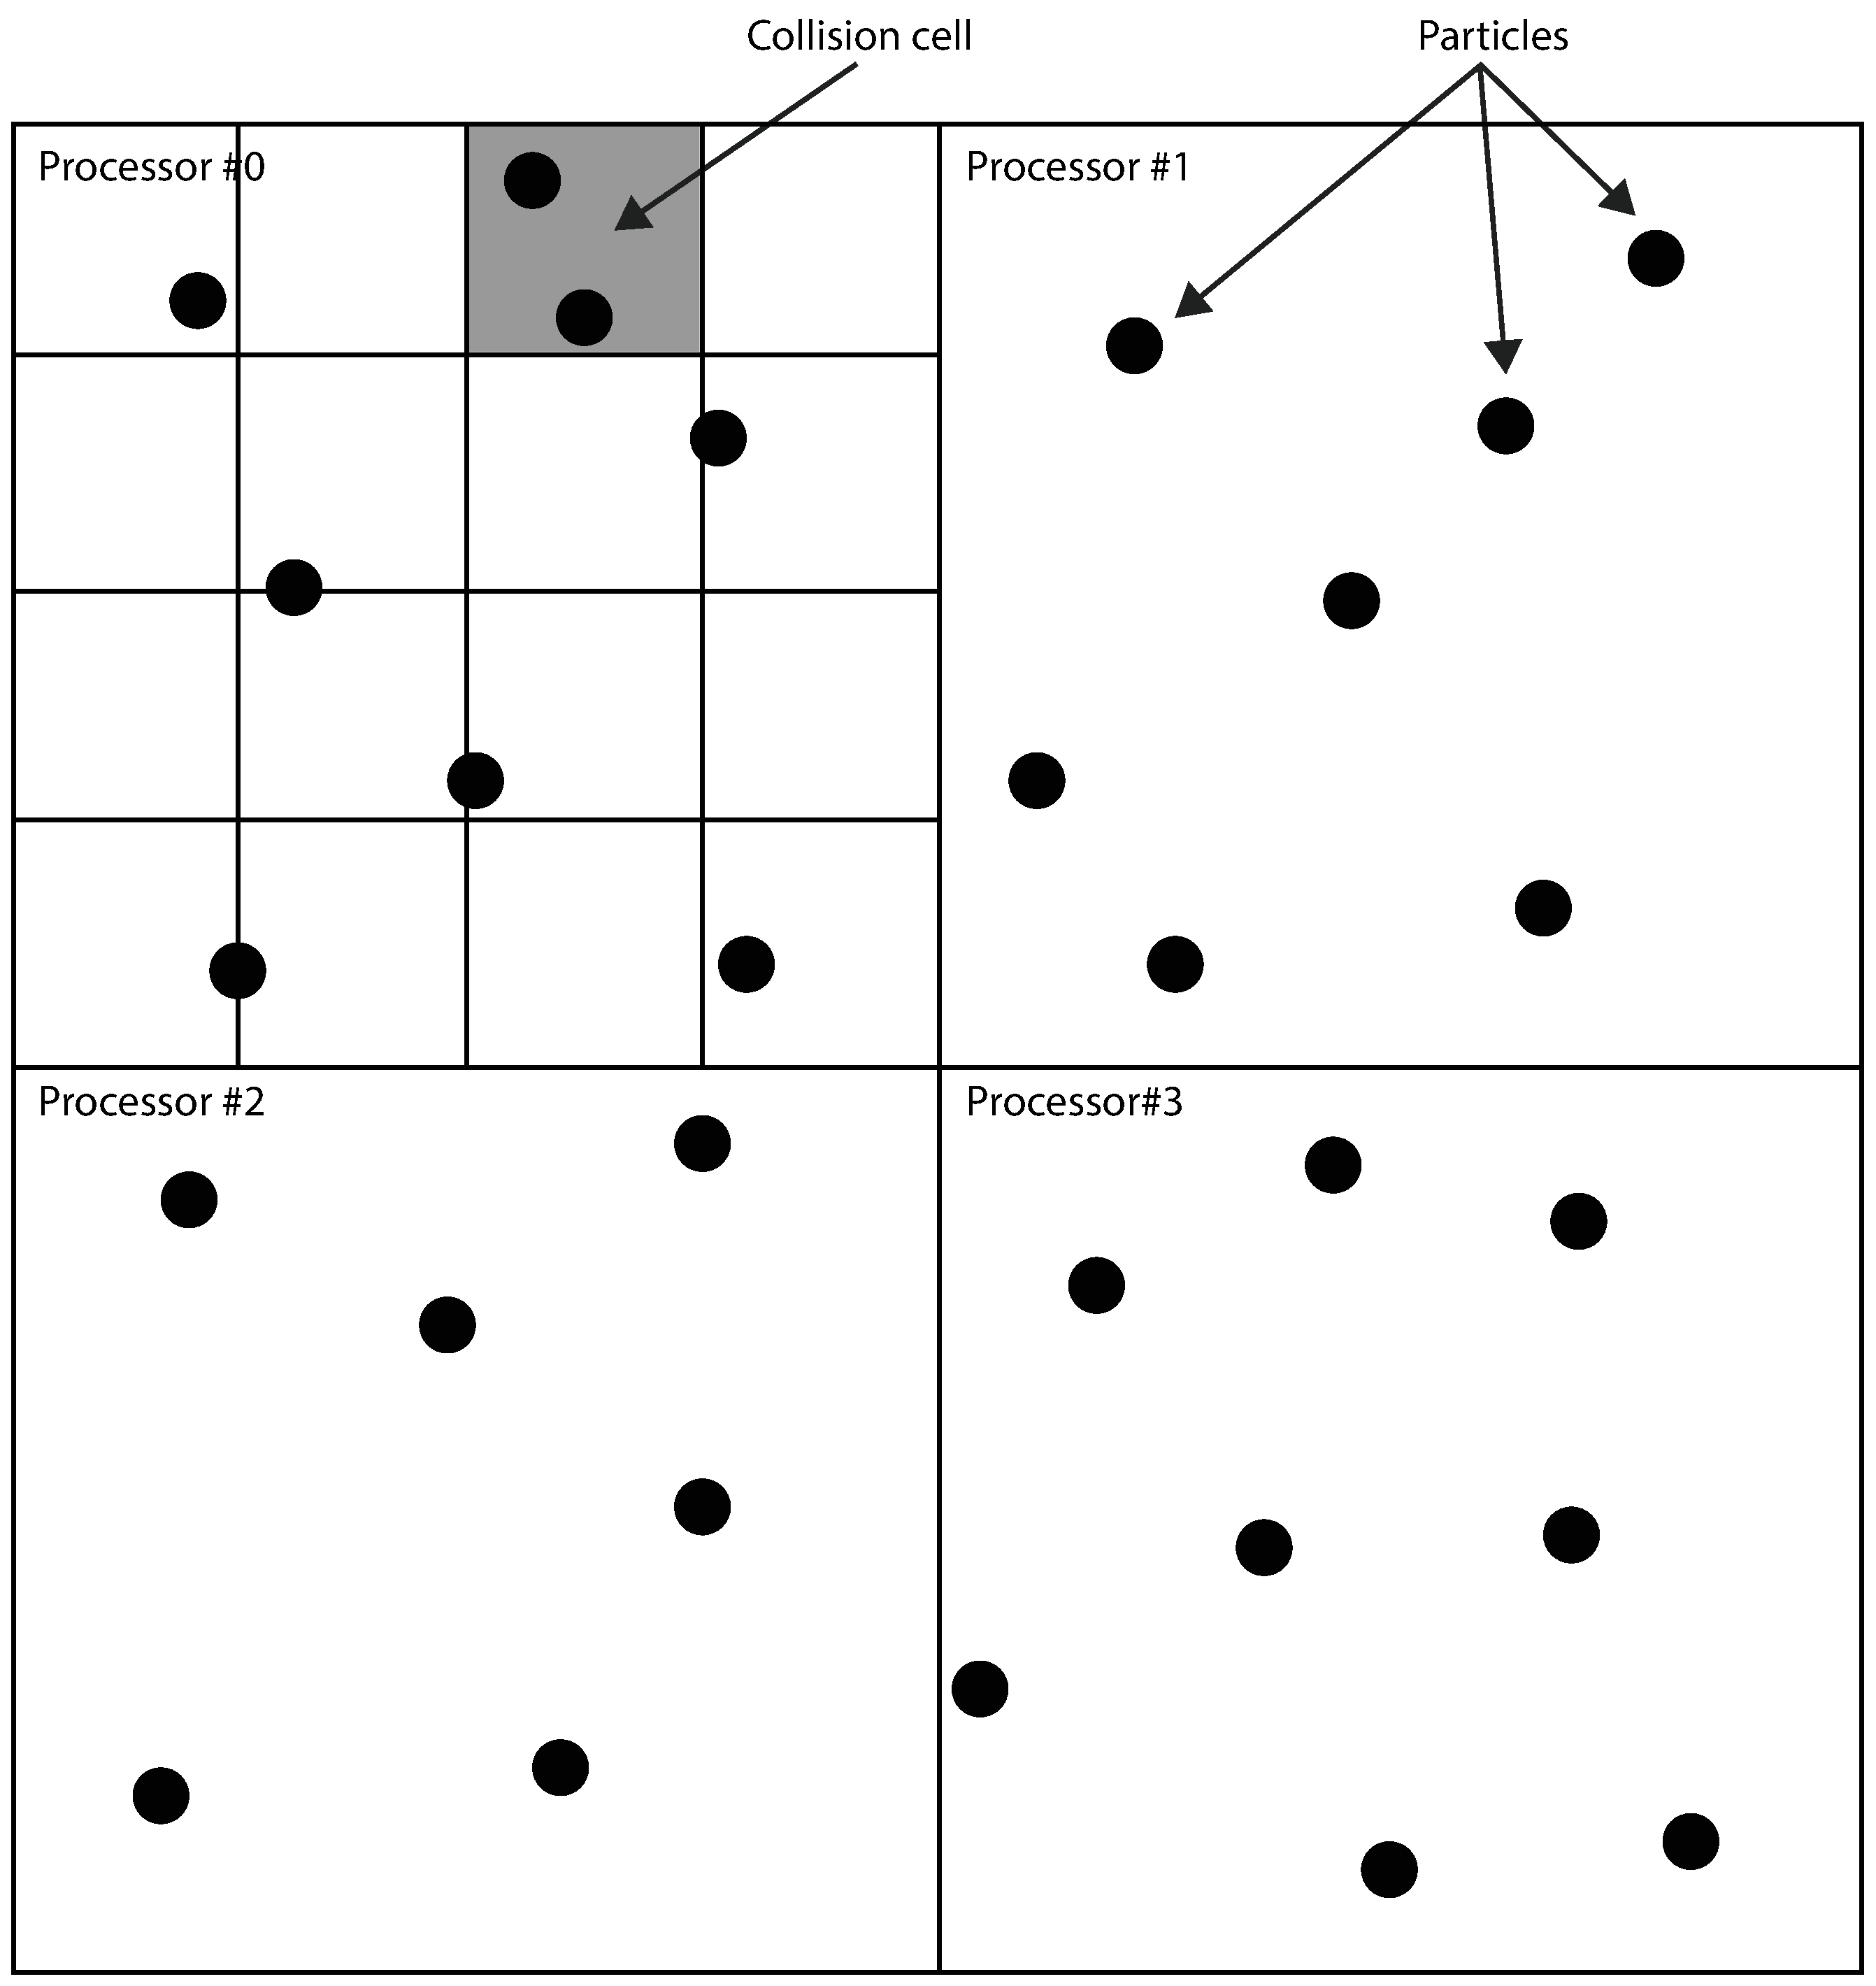
\includegraphics[width=\textwidth, trim=0cm 0cm 0cm 0cm, clip]{DSMC/figures/parallelization.eps}
\label{fig:dsmc_parallelization_1}
\end{center}
\caption{Illustration of how the spatial domain can be divided into four subdomains, each controlled by a processor. Each processor contains many particles that are placed in several collision cells (marked grey).}
\end{figure}
If we first assume that all the processors have full knowledge about the geometry of the full system, the only thing we have to take care of is when particles move from one processor to another. We have used (MPI) for the communcation between processors, and it is assumed that the reader is familiar with how MPI works. 
\subsection{Topological structure}
The processors are divided into a three dimensional grid with $(P_x, P_y, P_z)$ being the number of CPU's in each dimension yielding a total of $P = P_x\cdot P_y\cdot P_z$ processors. We can then use the grid coordinates $(p_x, p_y, p_z)$ to uniquely label the processors as shown in figure \ref{fig:dsmc_parallelization_2}.
\begin{figure}[h]
\begin{center}
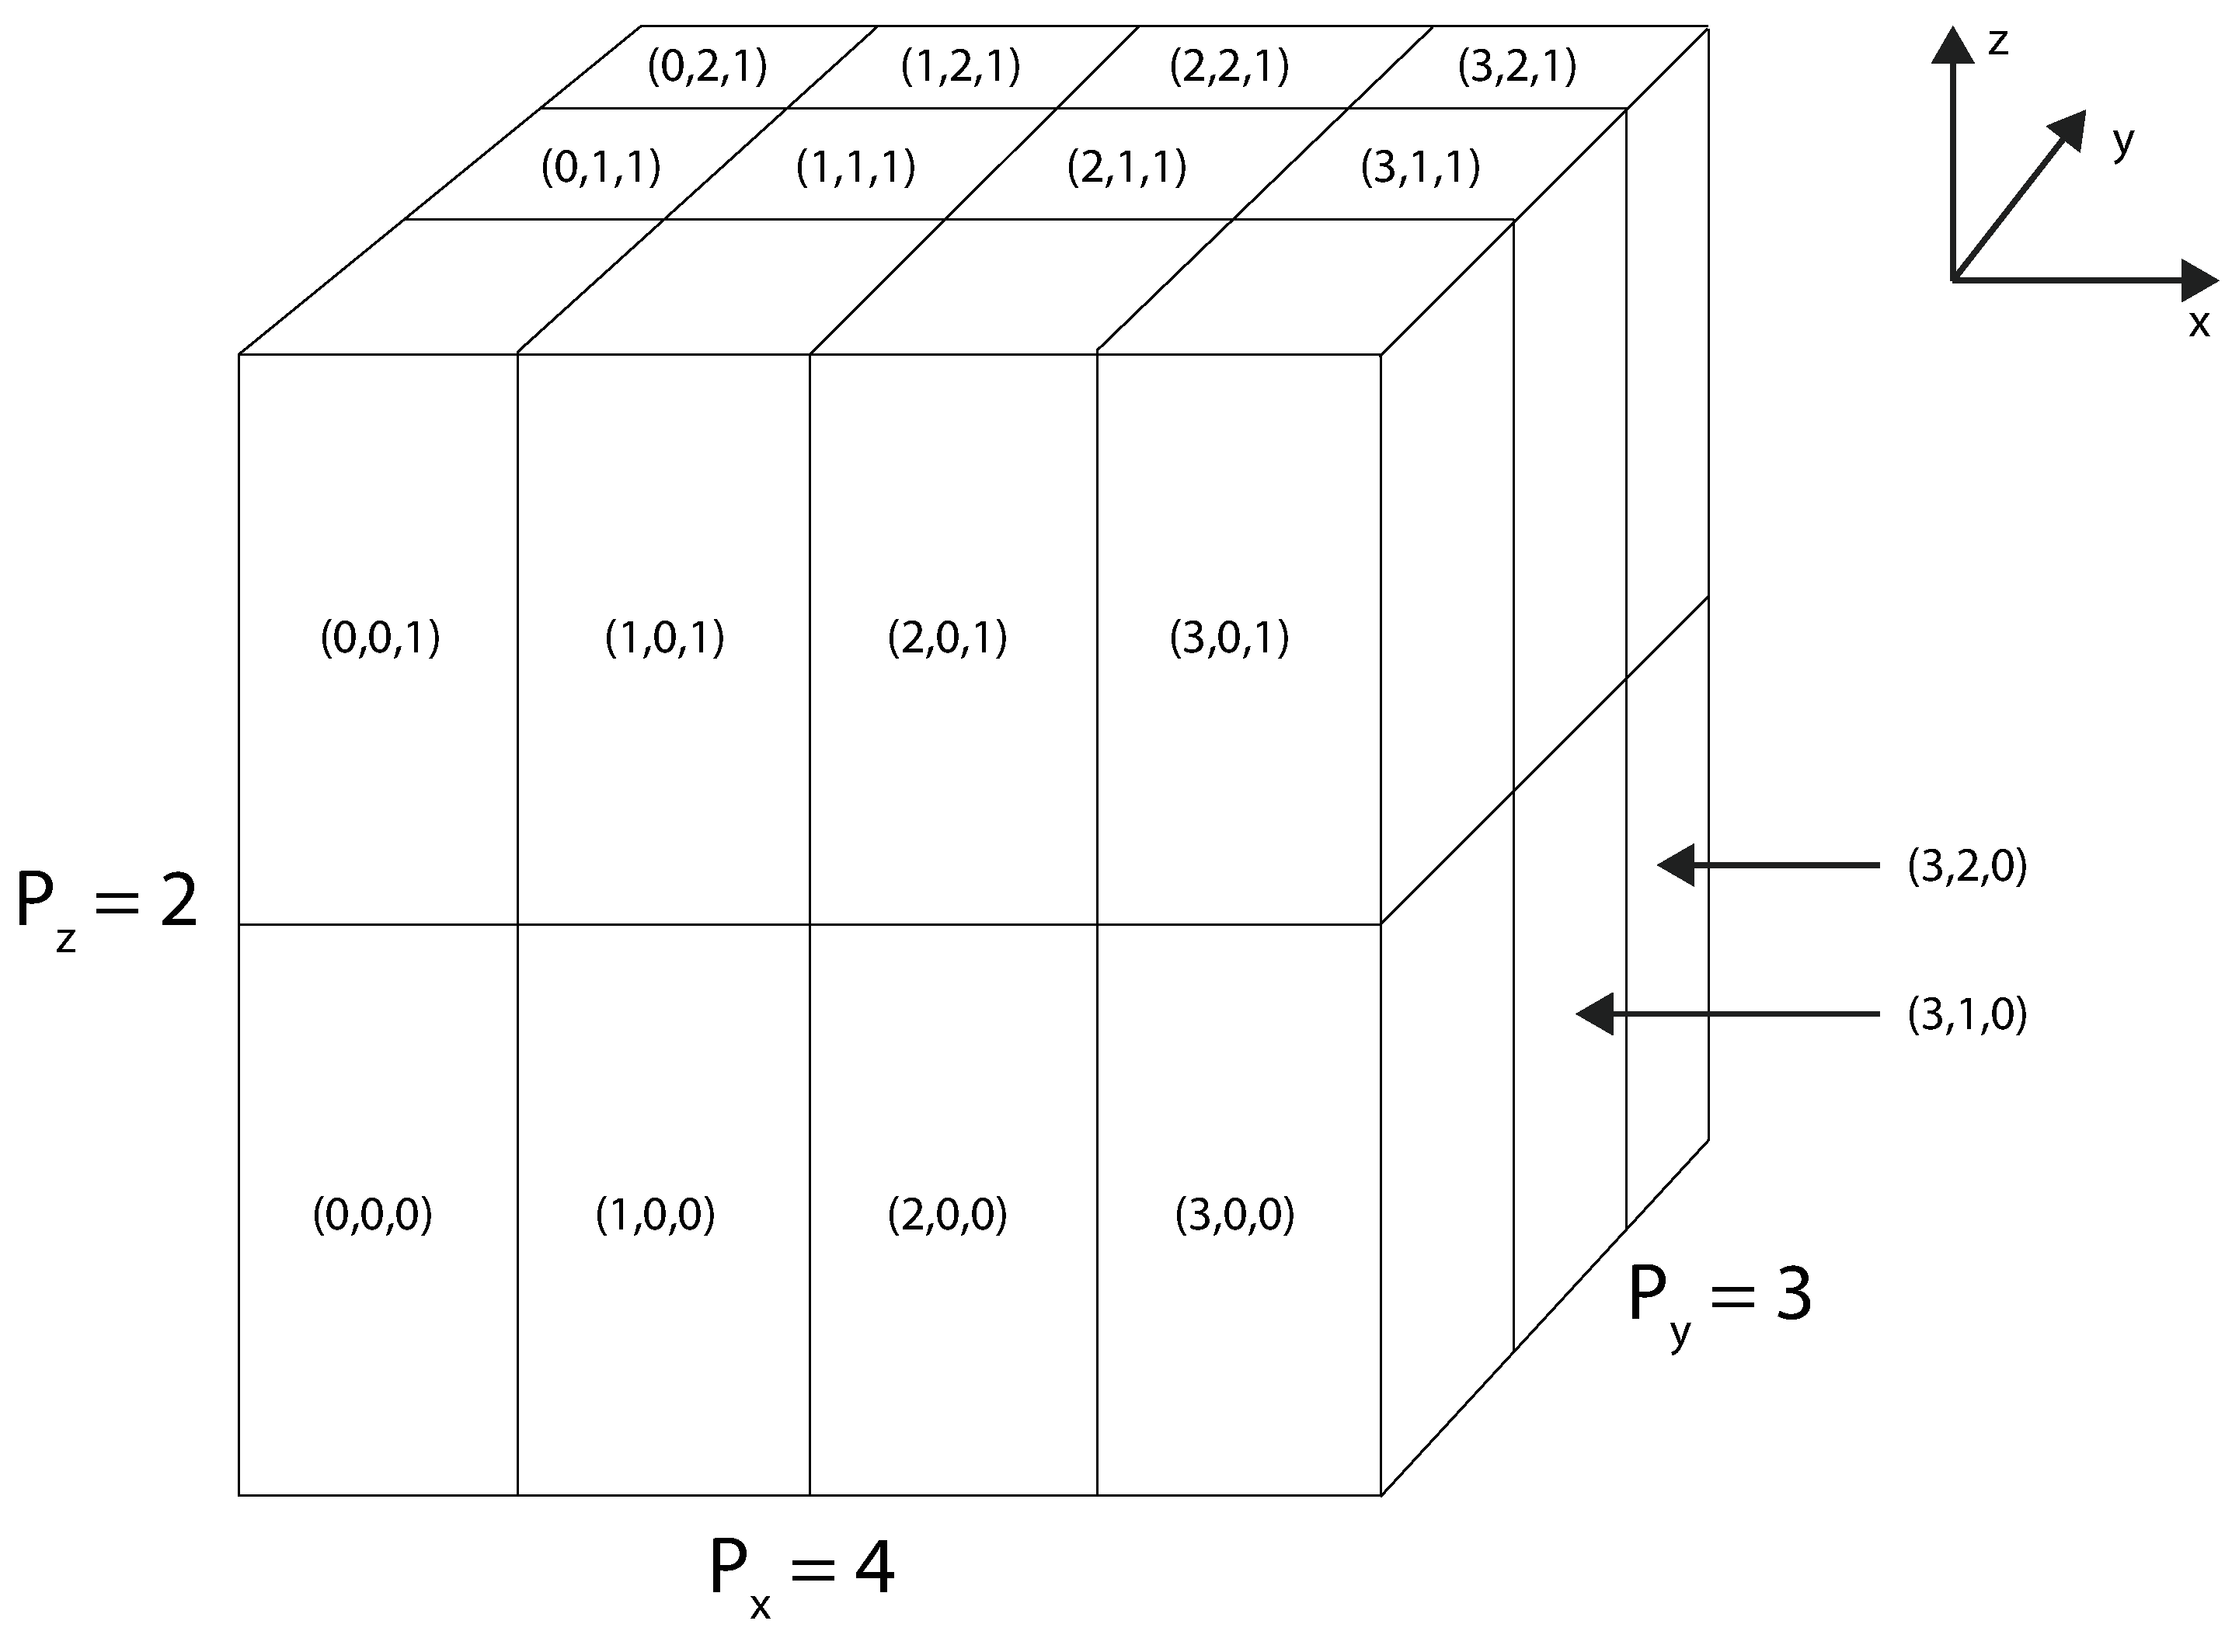
\includegraphics[width=\textwidth, trim=0cm 0cm 0cm 0cm, clip]{DSMC/figures/parallelization_node_configuration.eps}
\label{fig:dsmc_parallelization_2}
\end{center}
\caption{Processor labeling in a 3-dimensional grid. Each processor is uniquely identified through its coordinate $(p_x, p_y, p_z)$.}
\end{figure}
When starting a program with MPI, each process is provided a unique identification number $p$ in the range $[0, P-1]$ for $P$ processors. This can be mapped to the 3-dimensional grid coordinates through
\begin{align}
	\nonumber
	p_x(p) &= {p \over P_yP_z}\\
	\nonumber
	p_y(p) &= {p \over P_z} \bmod P_y\\
	p_z(p) &= p \bmod P_z
\end{align}
whereas the inverted mapping is 
\begin{align}
	p(p_x, p_y, p_z) = p_x\cdot P_zP_y + p_y\cdot P_z + p_z.
\end{align}
With the processor id $p$ given, it is easy to determine which subvolume this processor should control. If the system is of size $L^{(i)}$ in the $i$'th dimension, we can find the \textit{node length} $L_{\text{node}}^{(i)} \equiv l_i = L_i/P_i$. A processor with coordinates $(p_x, p_y, p_z)$ will control all particles with coordinates in the range
\begin{align}
	\nonumber
	x&\in[p_xl_x, (p_x+1)l_x\rangle\\
	\nonumber
	y&\in[p_yl_y, (p_y+1)l_y\rangle\\
	z&\in[p_zl_z, (p_z+1)l_z\rangle.
\end{align}
Collisions will be performed within the collision cells as before, but will obviously happen in parallel. 
\subsection{Exchanging particles}
A particle can move from one processor to one of the neighbouring 26 nodes through what is called the \textit{boundary layer}, the processor needs to send that information to the reciever. 